\subsection*{Summary}
\begin{frame}
    \frametitle{Summary}
    \begin{columns}[t]
        \begin{column}{0.5\linewidth}
            \begin{block}{AHTR Model Development for the FHR Benchmark}
                \textbf{Results Presented} 
                \begin{itemize}
                    \item FHR benchmark Phase I-A and I-B results
                    \item AHTR full assembly temperature model 
                \end{itemize}

                Through participation in the FHR benchmark, this dissertation contributes to 
                \textbf{deepening our understanding of the promising \gls{AHTR} technology}.
            \end{block}
        \end{column}
        \begin{column}{0.5\linewidth}
            \begin{block}{ROLLO Tool Development and AHTR Non-Conventional Design Optimization}
                \textbf{Results Presented}
                \begin{itemize}
                    \item \acrfull{ROLLO} tool 
                    \item AHTR Optimization for heterogeneous fuel distributions and wavy 
                    coolant channels 
                \end{itemize}
                
                By designing the ROLLO tool and demonstrating its success in 
                optimization of the \gls{AHTR} beyond classical input parameters, this dissertation 
                contributes to \textbf{optimization tool development for reactors of the future}.
            \end{block}
        \end{column}
    \end{columns}
\end{frame}

\subsection*{FHR Benchmark Specifications}
\begin{frame}
    \frametitle{FHR Benchmark Specifications}
    UIUC participates in the benchmark with OpenMC and using the ENDF/B-VII.1 material 
    cross section library
    \vspace{-0.2cm}
    \begin{table}
        \caption{OECD NEA's FHR Benchmark Phases 
        \cite{petrovic_benchmark_2021}.}
        \vspace{-0.25cm}
        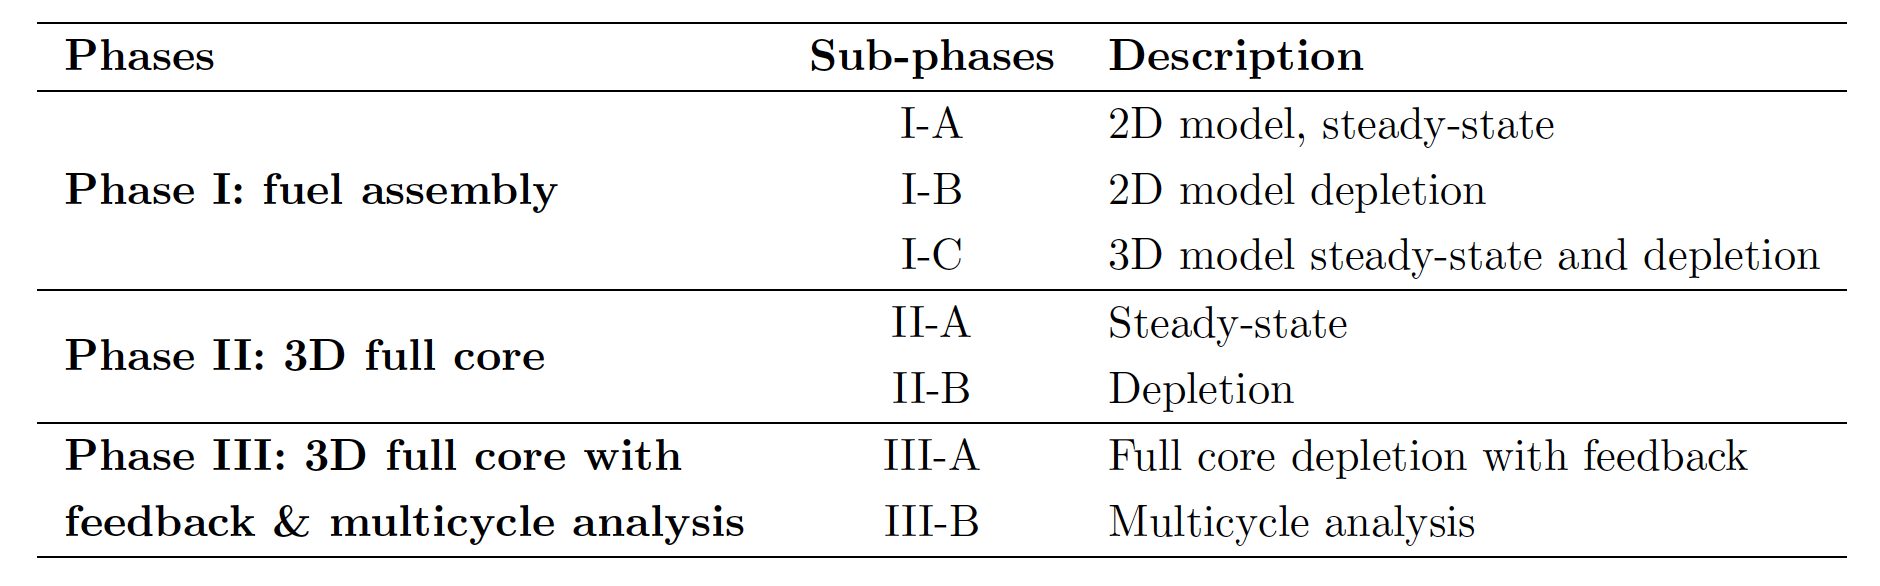
\includegraphics[width=0.7\linewidth]{figures/benchmark-phases.png} 
    \end{table}
    \vspace{-0.3cm}
    \begin{figure}[]
        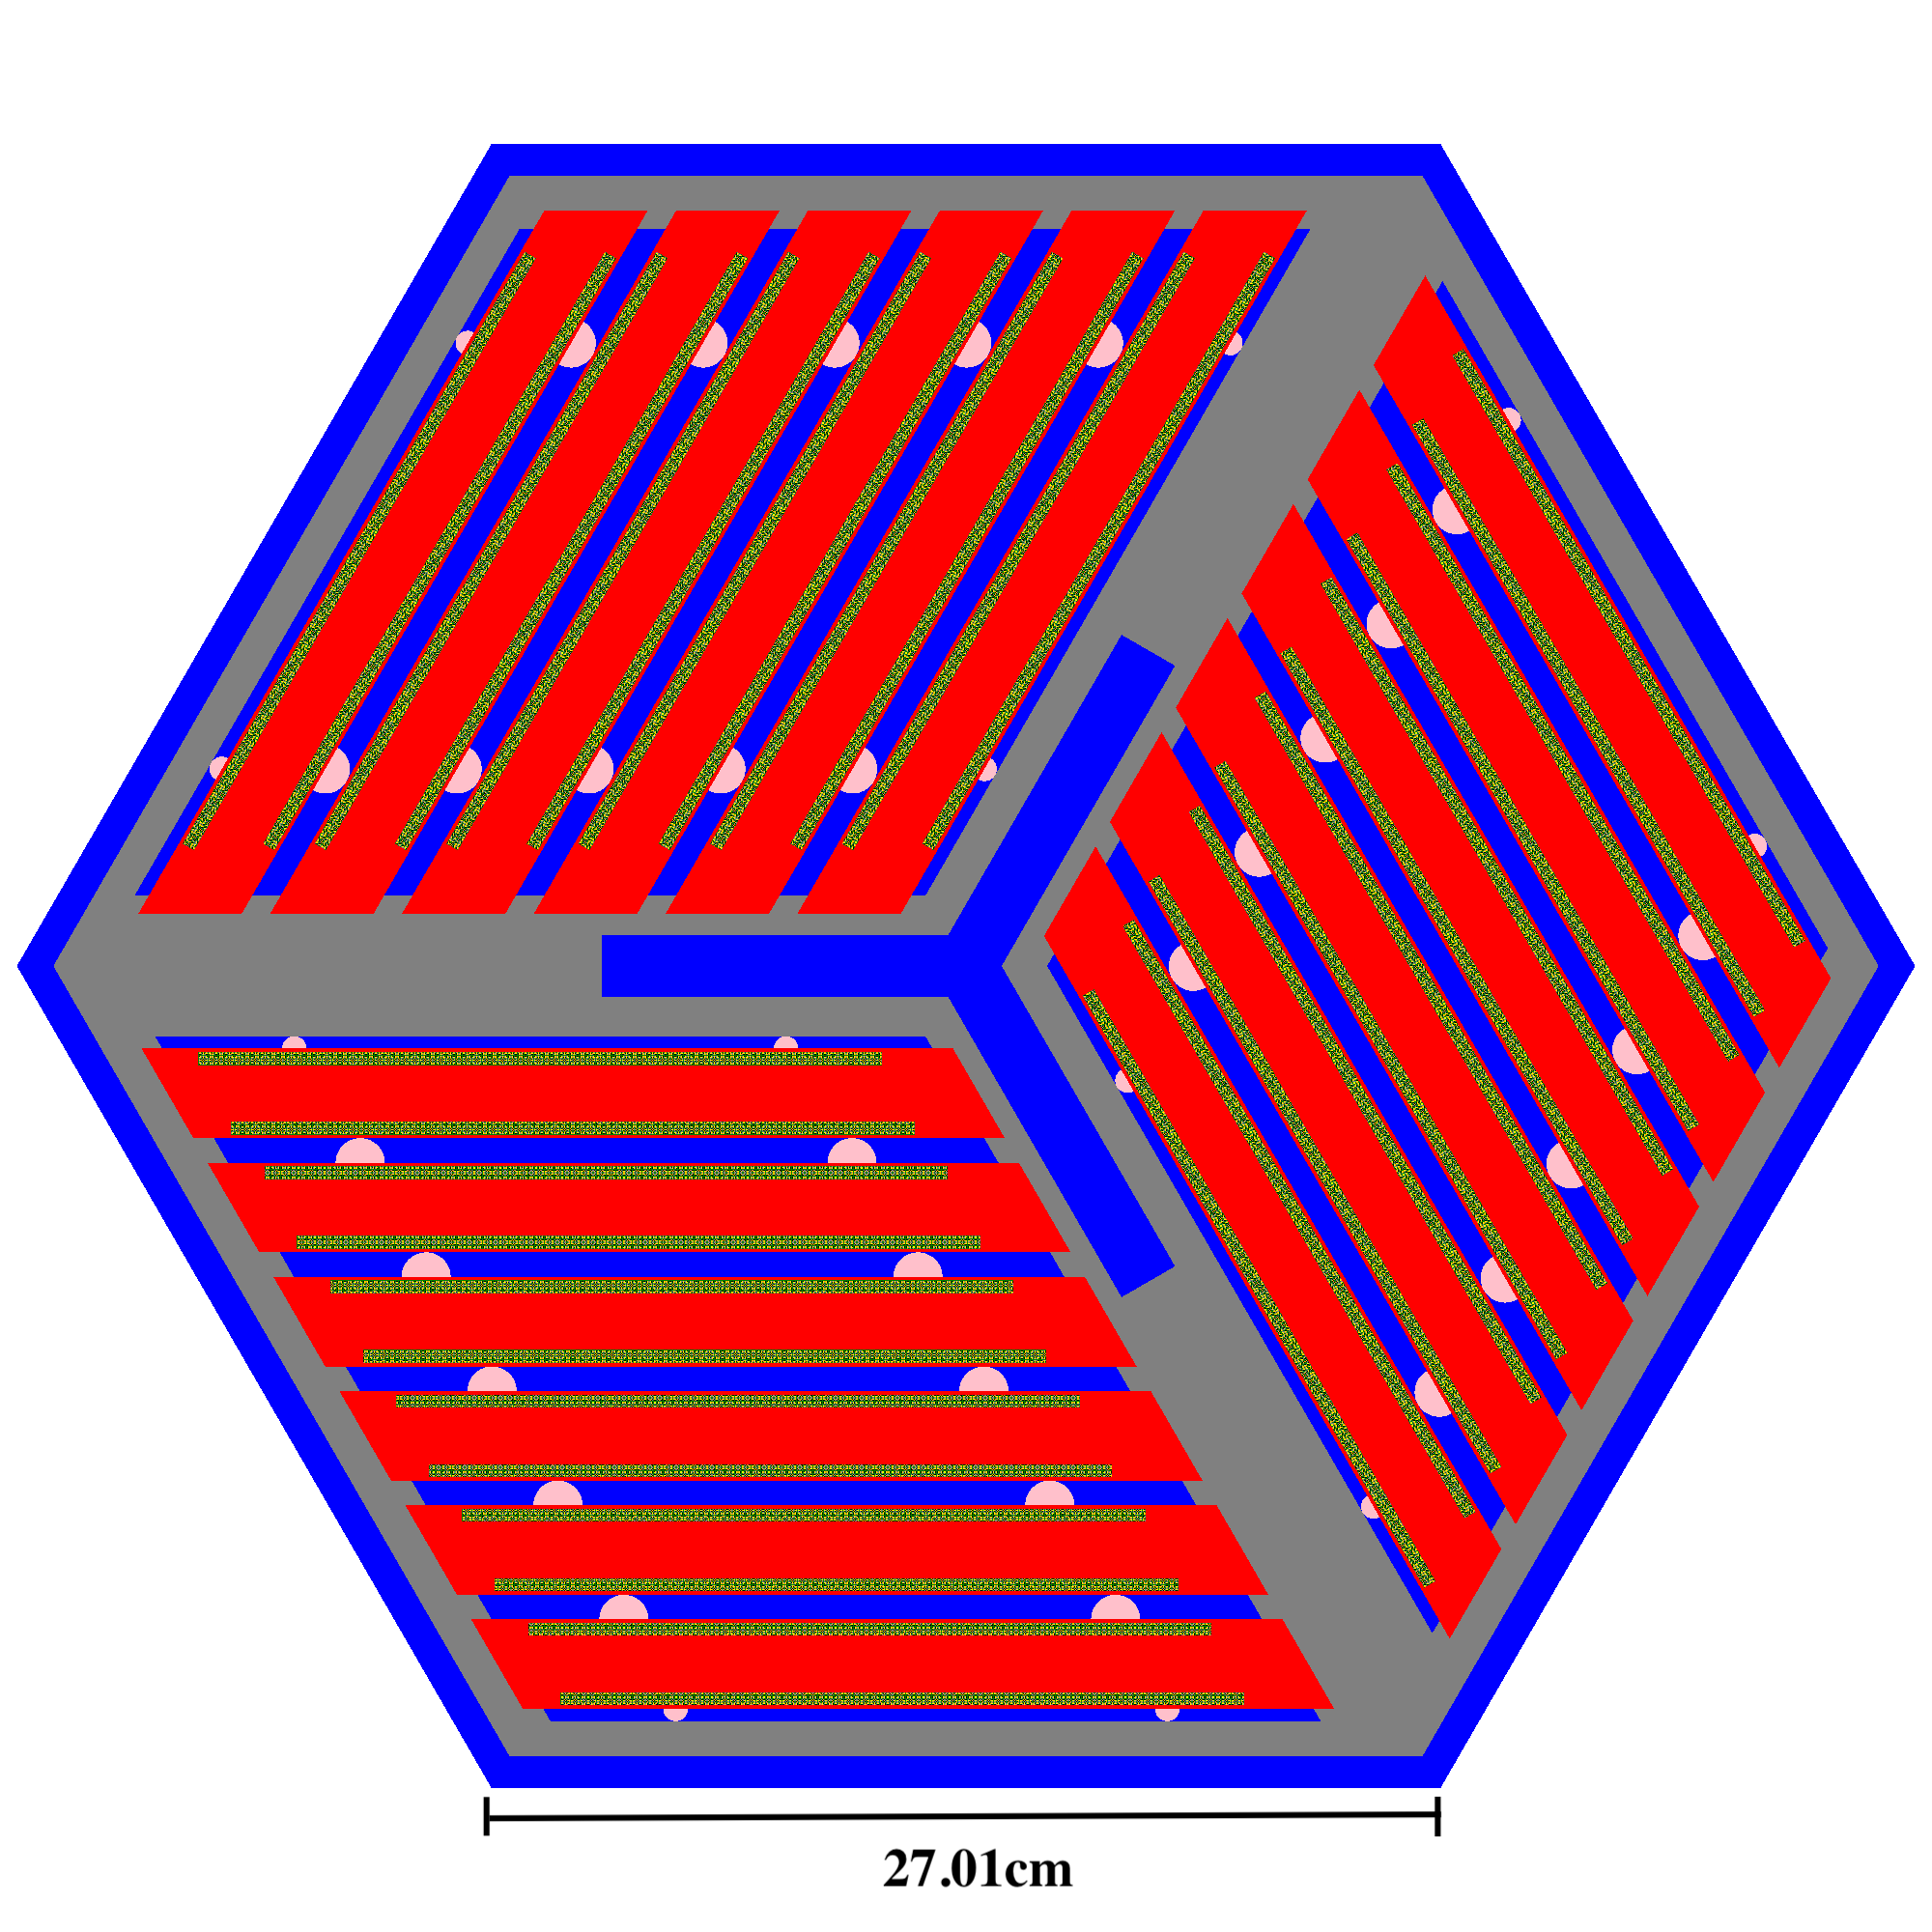
\includegraphics[width=0.27\linewidth]{../docs/figures/ahtr-fuel-element.png} 
        \vspace{-0.2cm}
        \caption{AHTR fuel assembly.}
    \end{figure}
\end{frame}

\begin{frame}
    \frametitle{FHR Benchmark Specifications}
    Only Phase I-A and I-B specifications have been released 
    \begin{table}
        \caption{Description of the \acrlong{FHR} benchmark Phase I-A cases 
        \vspace{-0.25cm}
        \cite{petrovic_benchmark_2021}.}
        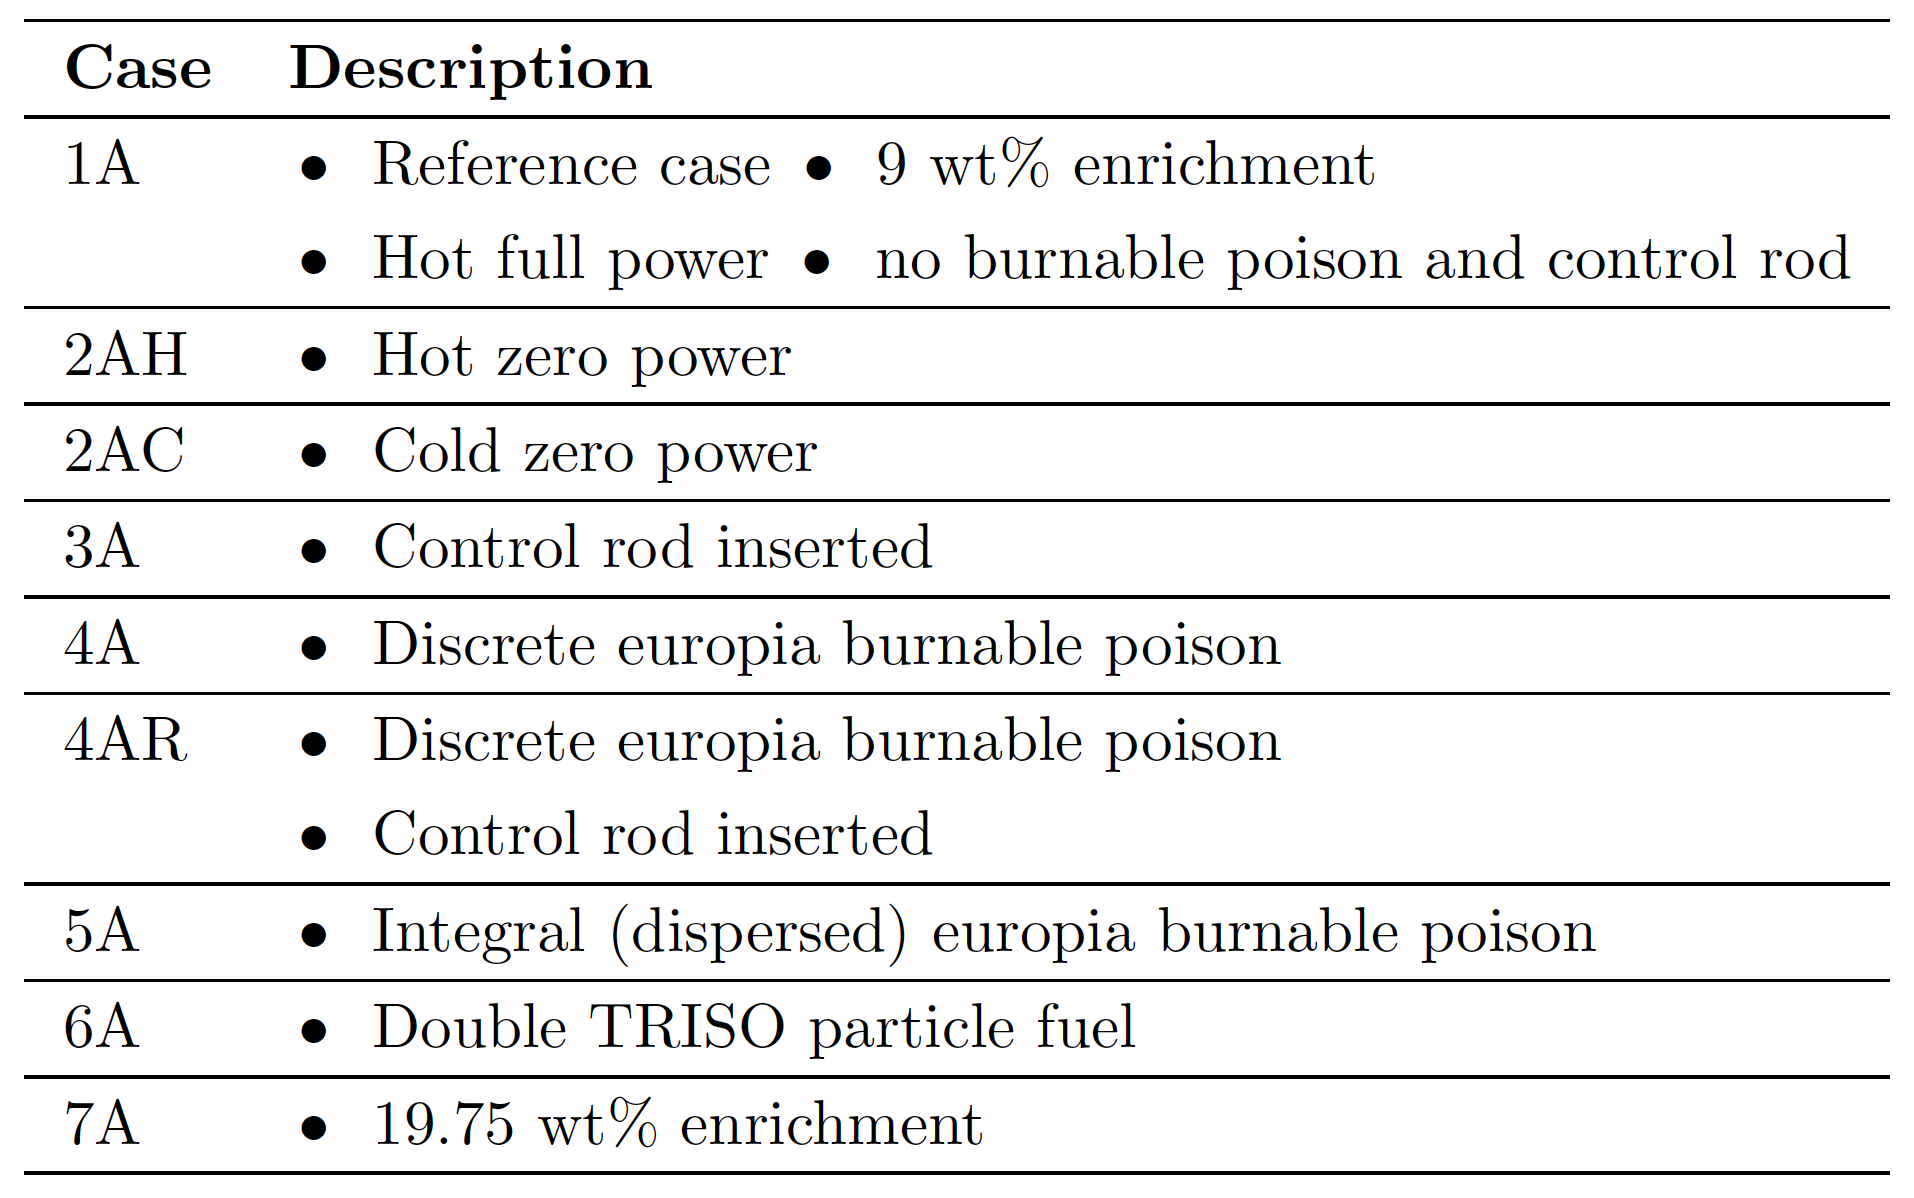
\includegraphics[width=0.8\linewidth]{figures/benchmark-cases.png} 
    \end{table}
    Benchmark participants must produce the following results for 
    the 9 cases: $k_{eff}$, reactivity coefficients ($\beta_{eff}$, 
    $\alpha_D$, $\alpha_{T, FliBe}$, $\alpha_M$), fission source distribution, 
    neutron flux distribution, fuel assembly averaged neutron spectrum
\end{frame}

\begin{frame}
    \frametitle{AHTR Self-Shielding Effects}
    The self-shielding neutrons are more likely absorbed at the fuel regions at the 
    plank's sides, near the pure graphite structure moderating regions. 
    The outer sides of the plank absorb these neutrons and geometrically shield the 
    plank's center from neutron flux, leading to a relatively lower group 4 thermal 
    flux in the plank's center for the constant TRISO distribution. 
\end{frame}

\subsection*{Key Neutronics Parameters Verification}
\begin{frame}
    \frametitle{AHTR Temp Model $k_{eff}$ and Reactivity Coefficients Verification}
        \begin{table}
            \caption{$k_{eff}$ and reactivity comparison.}
            \vspace{-0.2cm}
            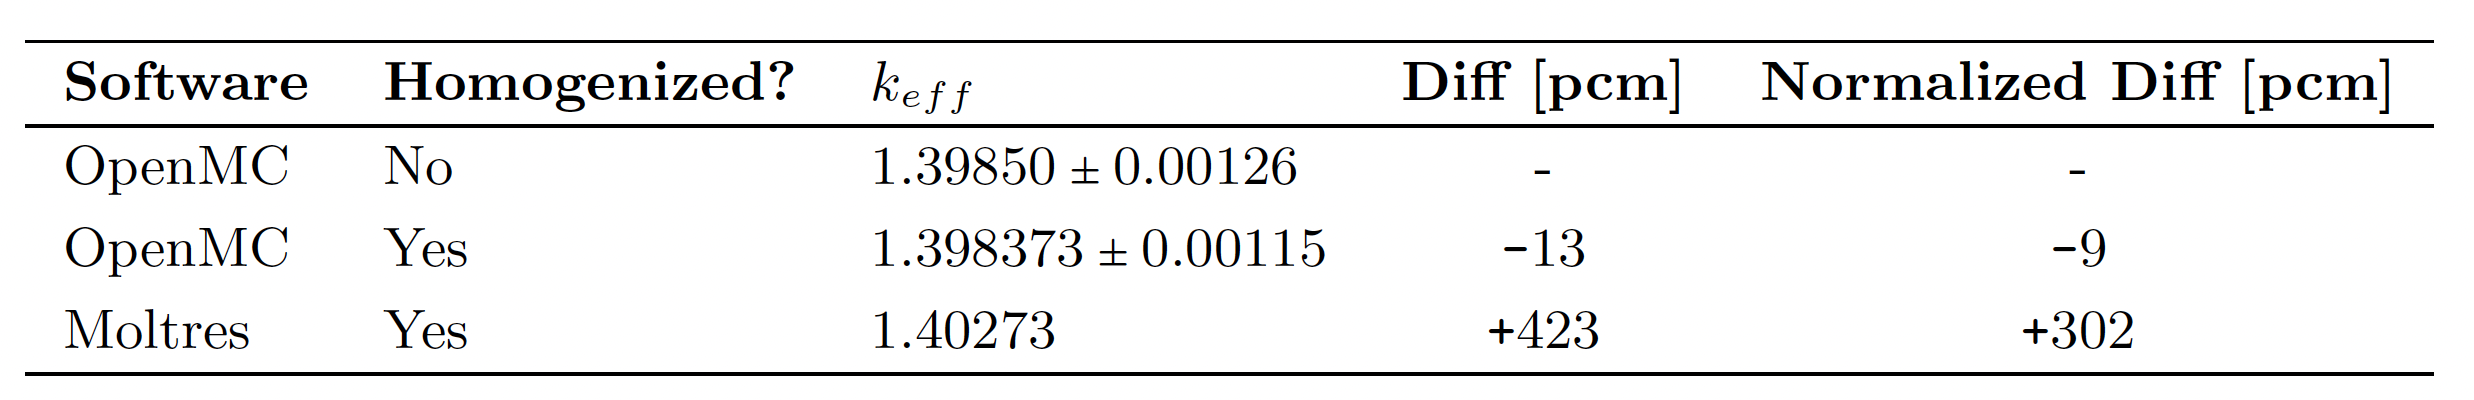
\includegraphics[width=0.9\linewidth]{figures/benchmark-keff.png}
        \end{table}
        The 13pcm $k_{eff}$ and 6pcm reactivity diff, between
        continuous and homogenized OpenMC simulations are within uncertainty, showing 
        that \textbf{selected spatial homogenizations and energy discretizations are 
        acceptable.}
        The Moltres simulation shows a 423pcm diff in $k_{eff}$ and 216pcm 
        diff in reactivity.
        \begin{table}
            \caption{Reactivity coefficients comparison.}
            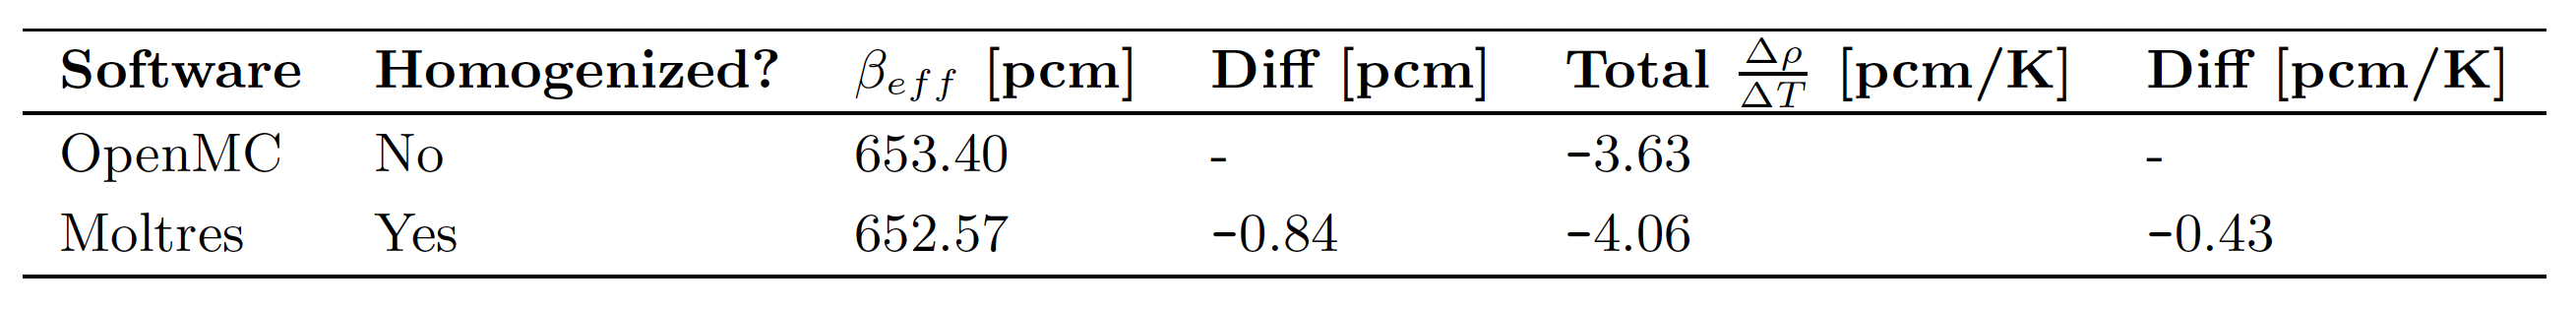
\includegraphics[width=0.85\linewidth]{figures/benchmark-coeff.png}
        \end{table}
        \textbf{Good agreement} for Moltres' delayed neutron fraction ($\beta_{eff}$) and 
        temperature reactivity feedback ($\frac{\Delta \rho}{\Delta T}$)
\end{frame}

\begin{frame}
    \frametitle{AHTR Temp Model Flux Verification}
    \begin{columns}
    \begin{column}{0.7\textwidth}
    \begin{figure}[]
        \centering
        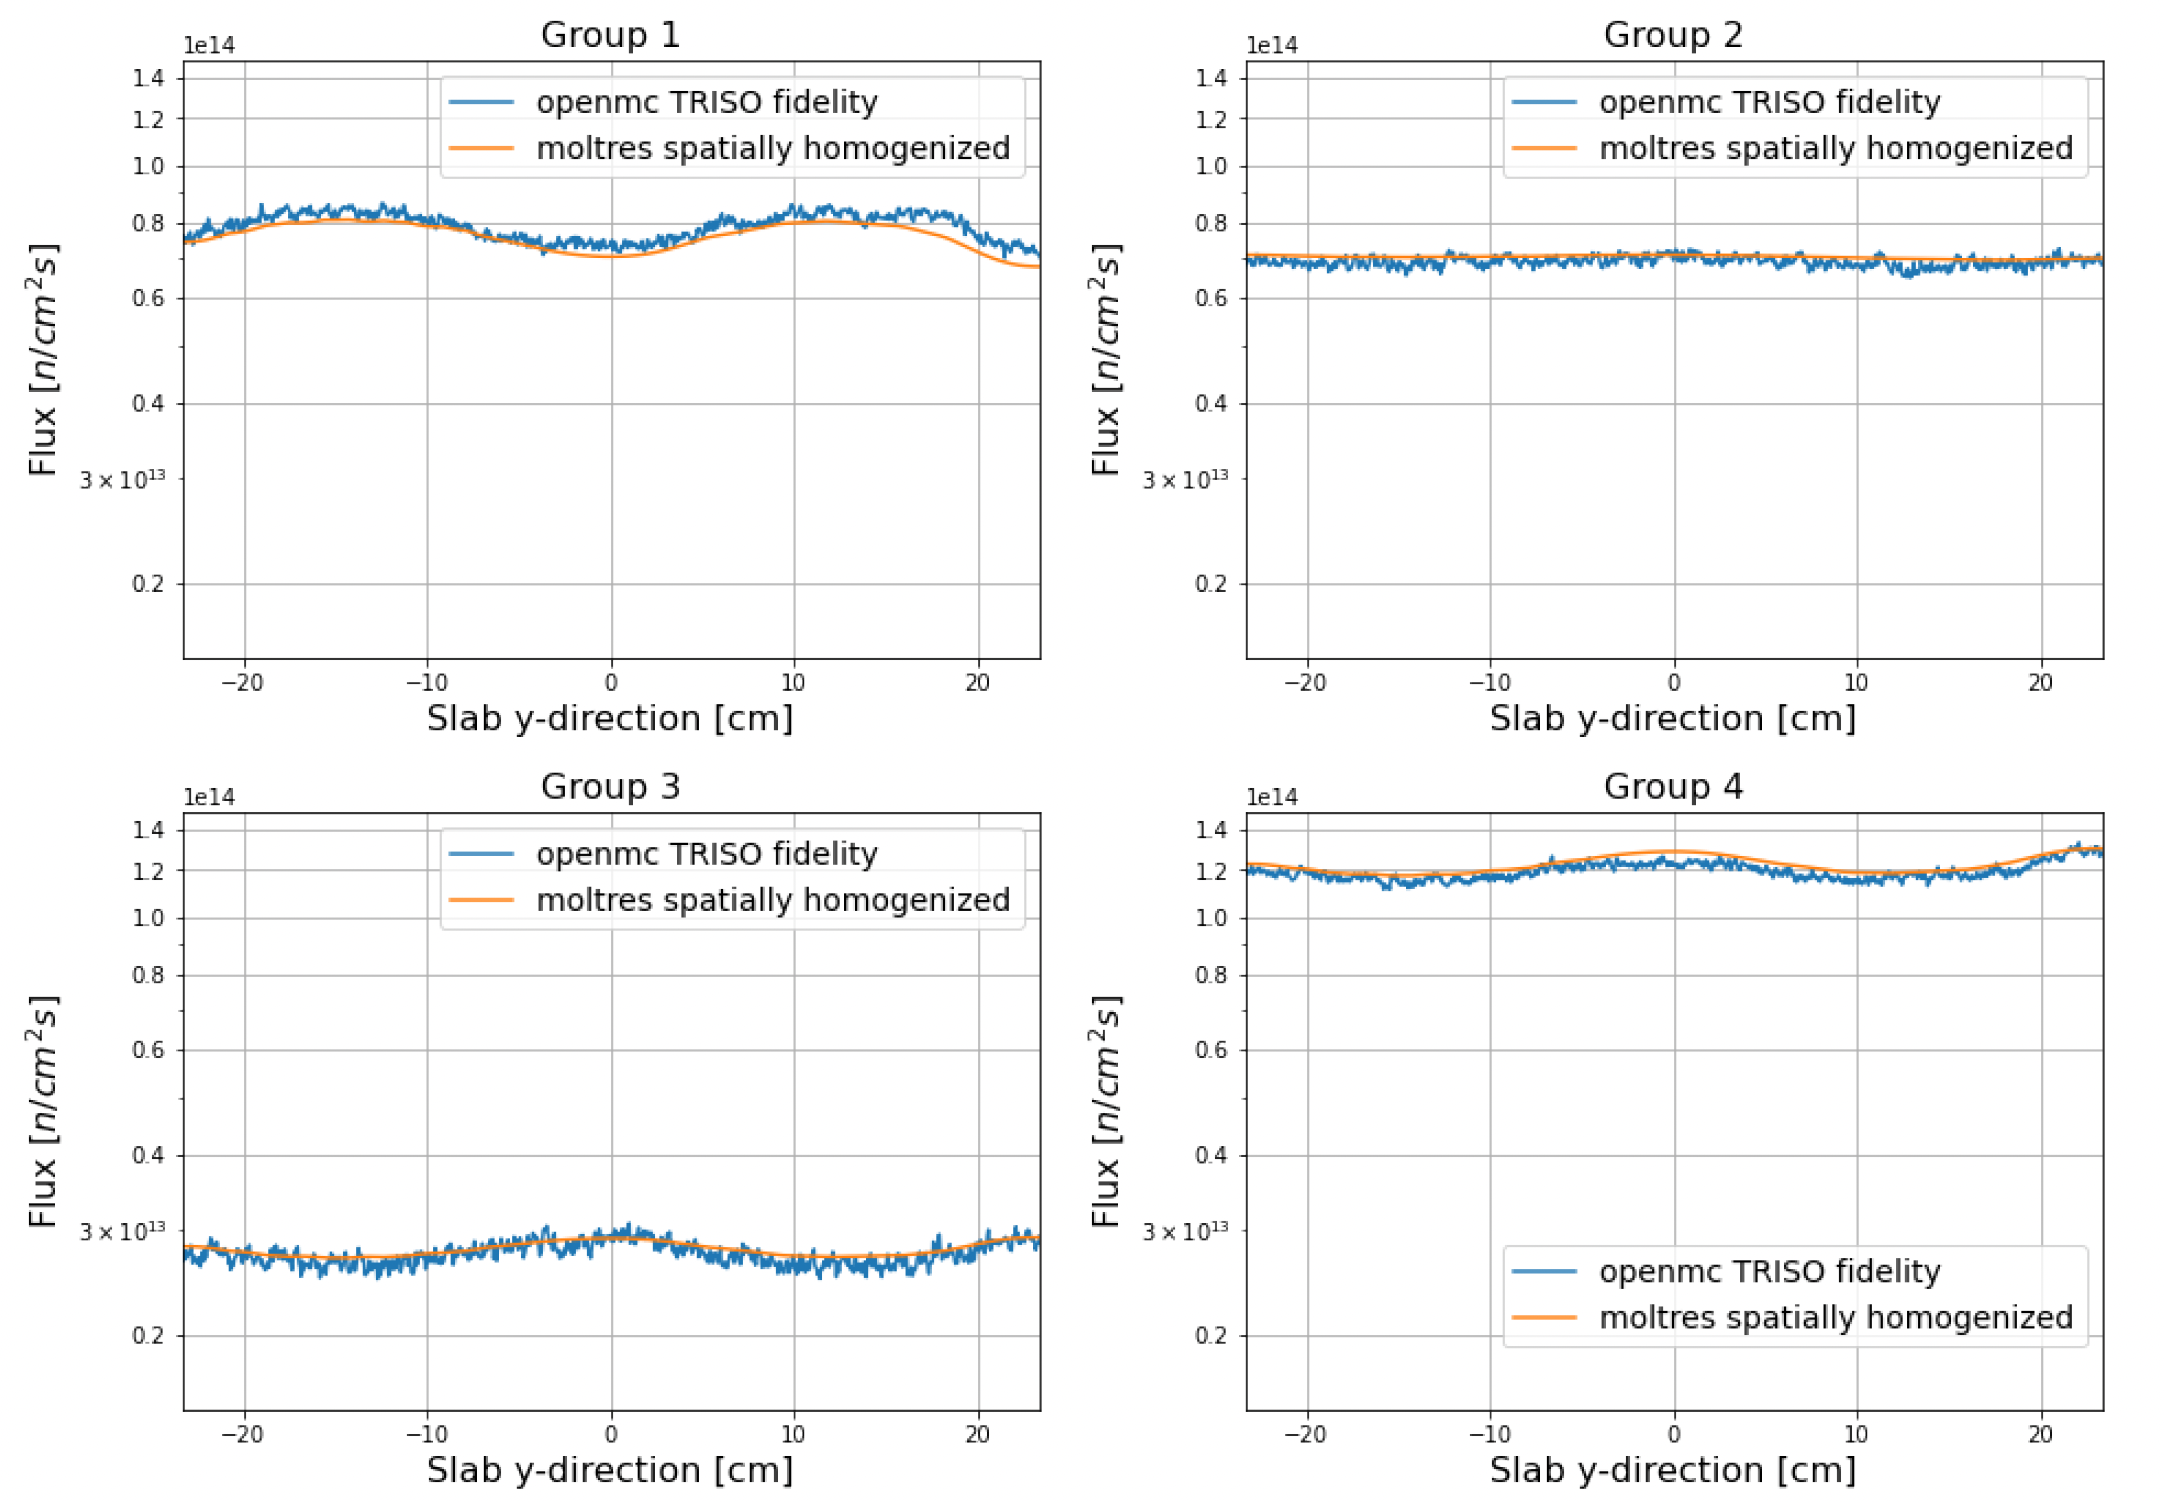
\includegraphics[width=\linewidth]{figures/benchmark-flux.png} 
        \caption{4-group flux distribution comparison.}
    \end{figure}
    \end{column}
    \begin{column}{0.3\textwidth}
        2-norm Diff [\%]
        \begin{itemize}
            \item Group 1: 0.13\% 
            \item Group 2: 0.08\% 
            \item Group 3: 0.10\% 
            \item Group 4: 0.09\%
        \end{itemize}
        Max Diff [\%]
        \begin{itemize}
            \item Group 1: -10.57\% 
            \item Group 2: +7.58\% 
            \item Group 3: +8.96\% 
            \item Group 4: +6.97\%
        \end{itemize}
    \end{column}
    \end{columns}
\end{frame}

\begin{frame}
    \frametitle{AHTR Temp Model Neutron Energy Spectrum Verification}
            \begin{figure}[]
                \centering
                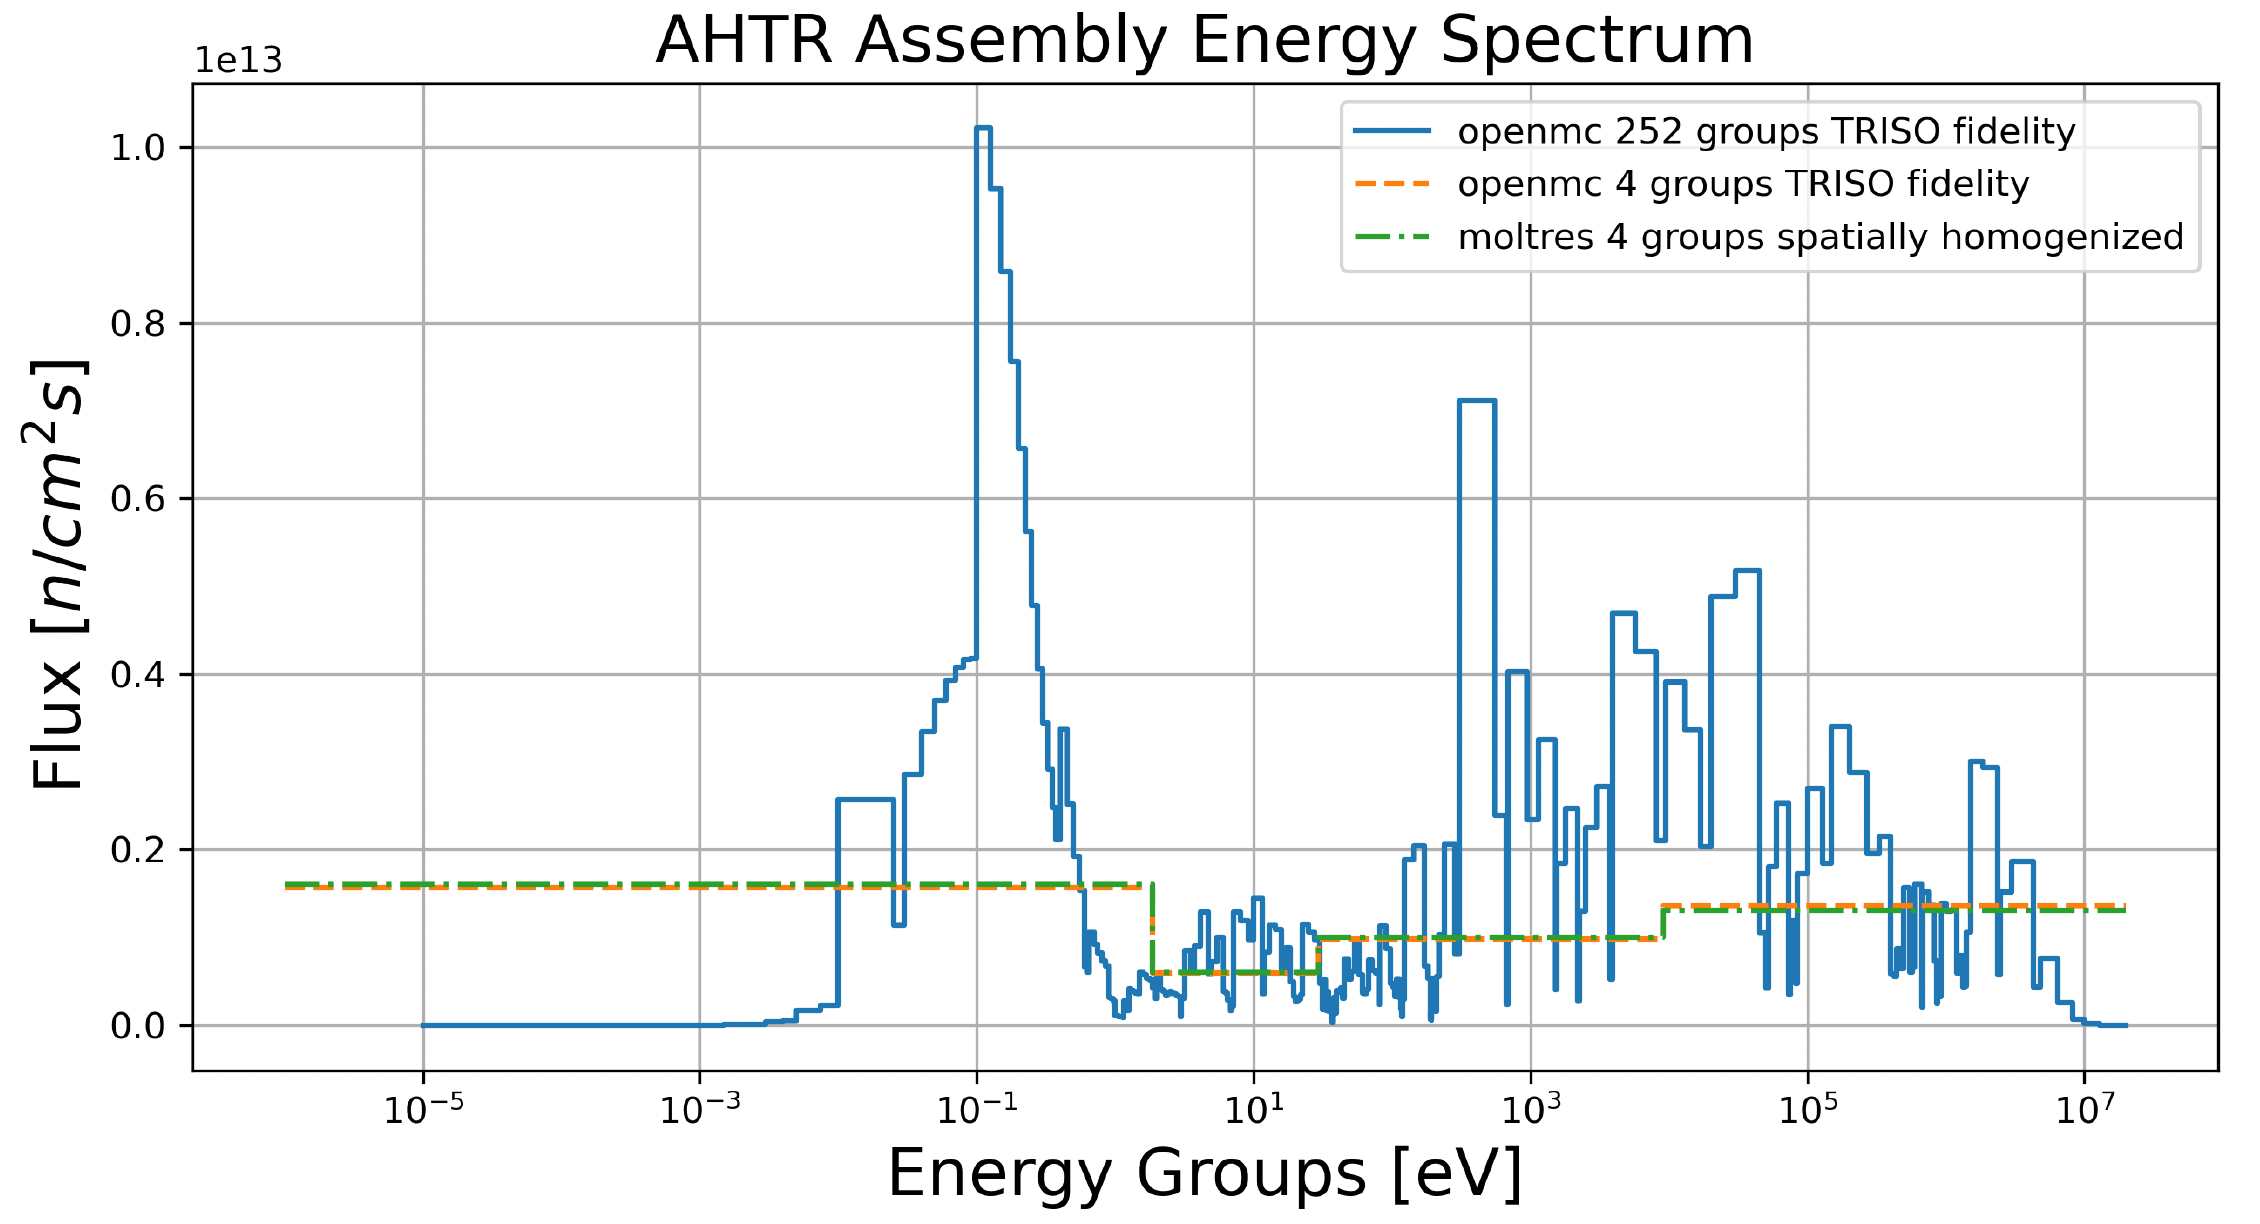
\includegraphics[width=0.75\linewidth]{figures/benchmark-spectrum.png} 
                \caption{Neutron Energy Spectrum Comparison.}
            \end{figure}
        \textbf{Good agreement} between OpenMC and Moltres models 4-group spectrums.
\end{frame}

\subsection{ROLLO Verification}
\begin{frame}
    \frametitle{ROLLO Successfully Verified with $^{239}Pu$ Critical Bare Sphere}
    \begin{figure}
        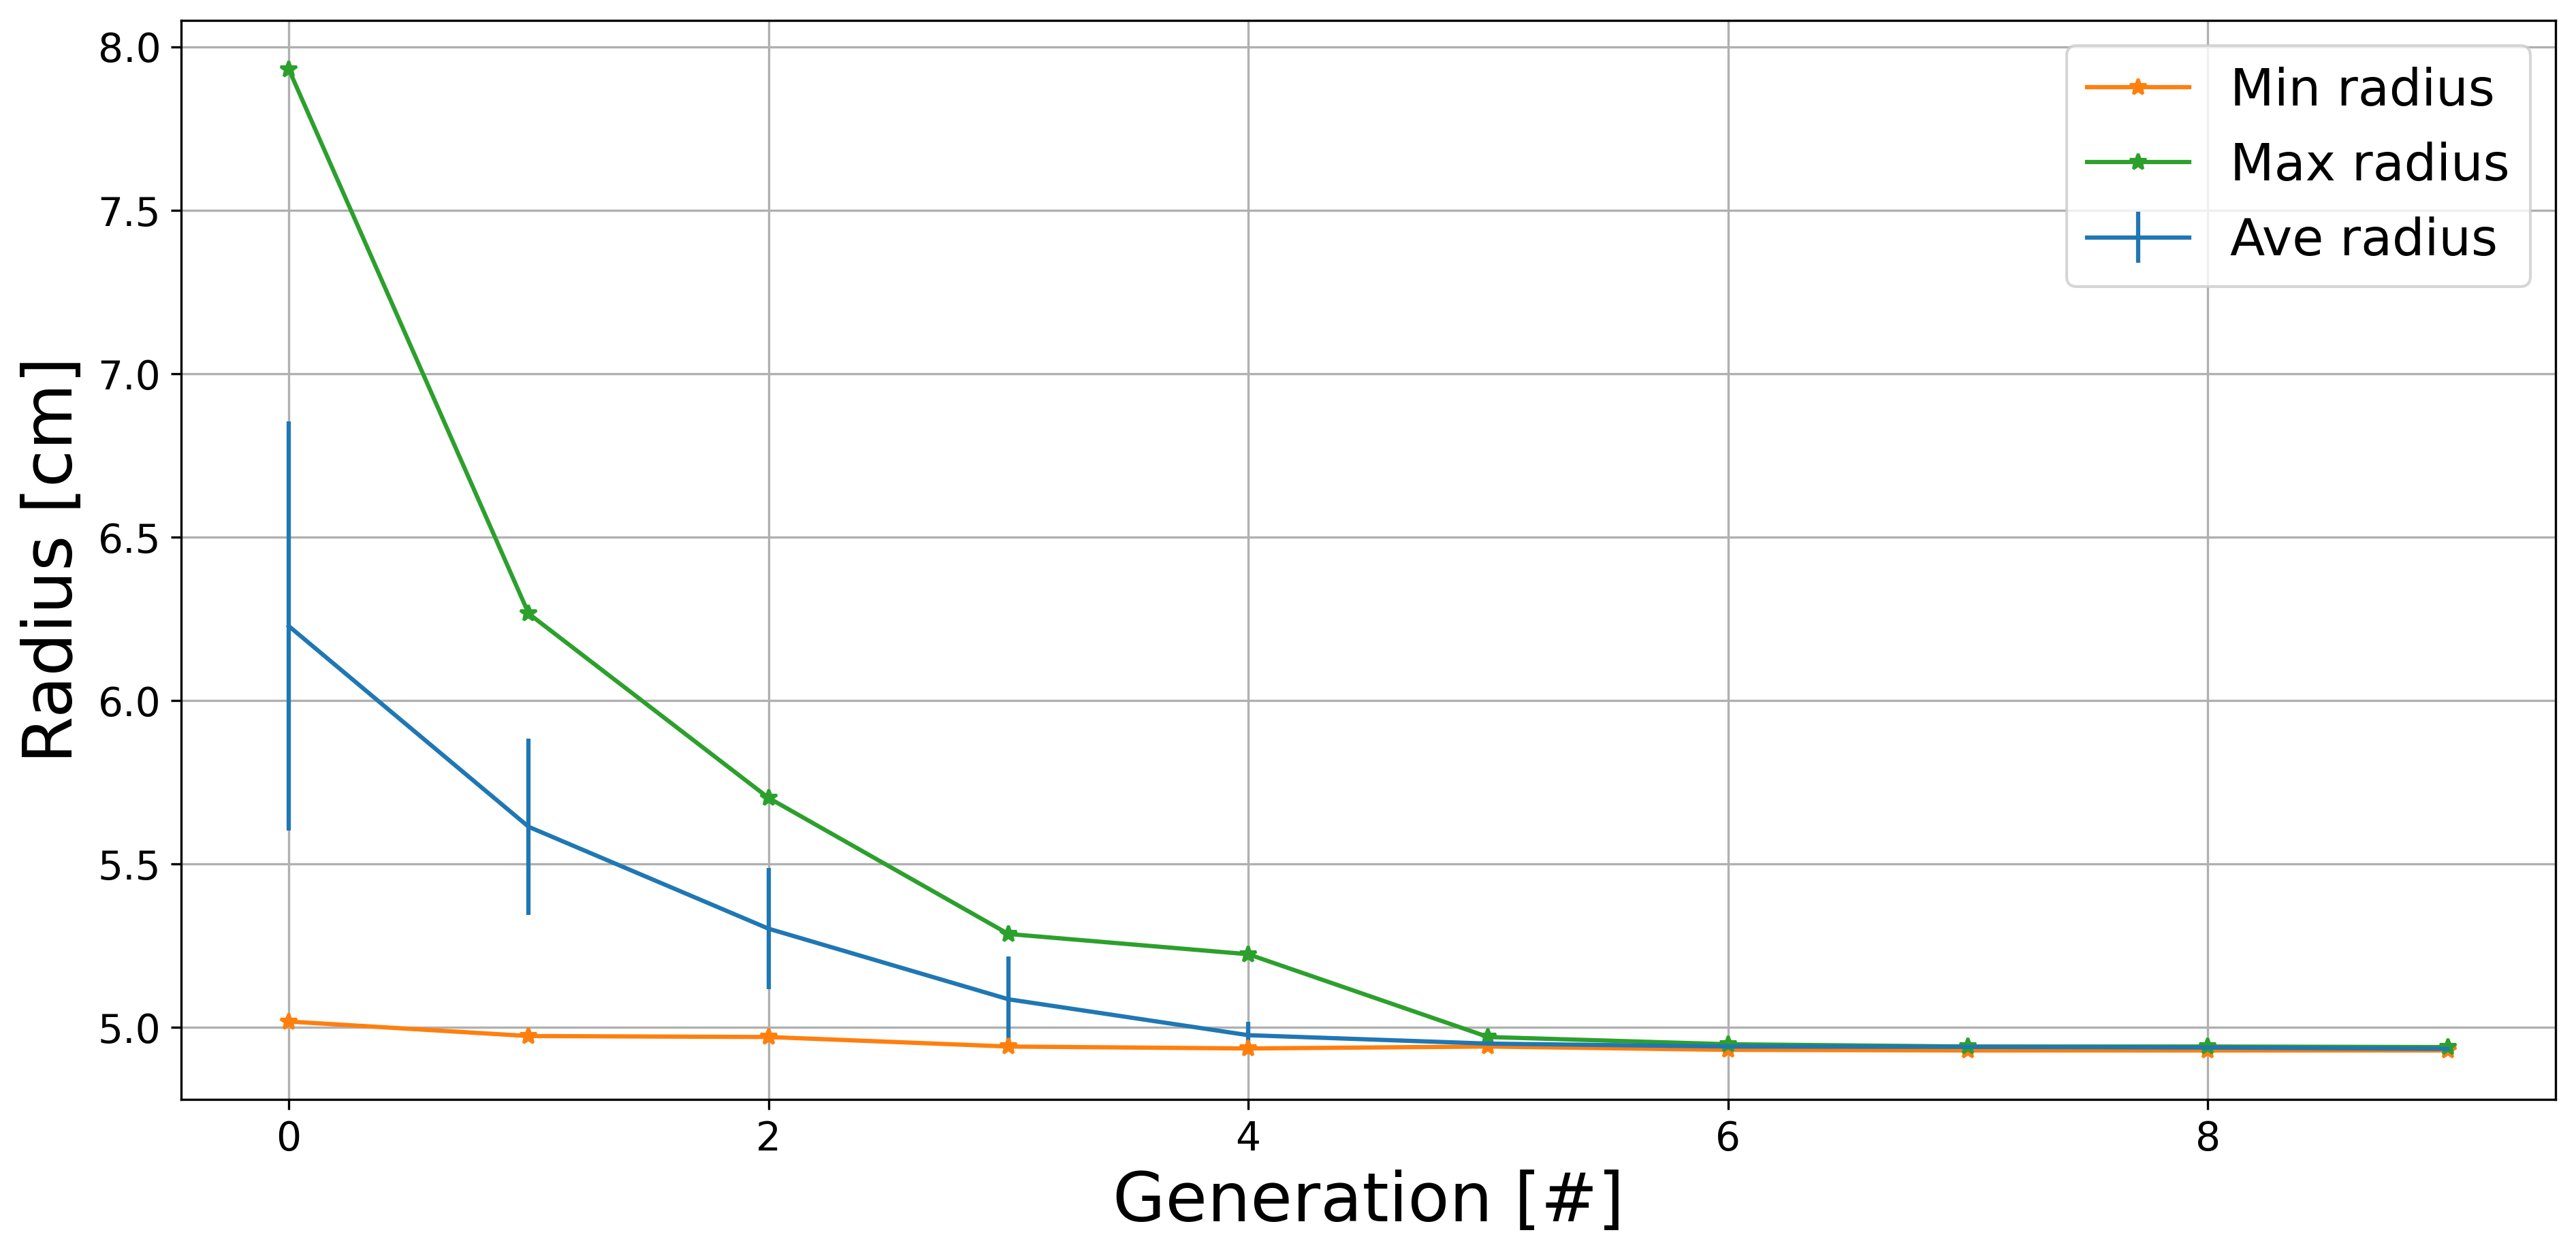
\includegraphics[width=0.85\linewidth]{../docs/figures/radius-convergence.png} 
        \caption{Results for each generation for \gls{ROLLO}'s genetic algorithm 
        optimization to the find the critical radius of a  $^{239}Pu$ bare sphere.}
    \end{figure}
    \vspace{-0.2cm}
    \textbf{ROLLO successfully finds the critical radius of the $^{239}Pu$ bare sphere 
    to be 4.9856cm.}
\end{frame}

\begin{frame}
    \frametitle{ROLLO $^{239}Pu$ Critical Bare Sphere Input File}
    \begin{figure}
        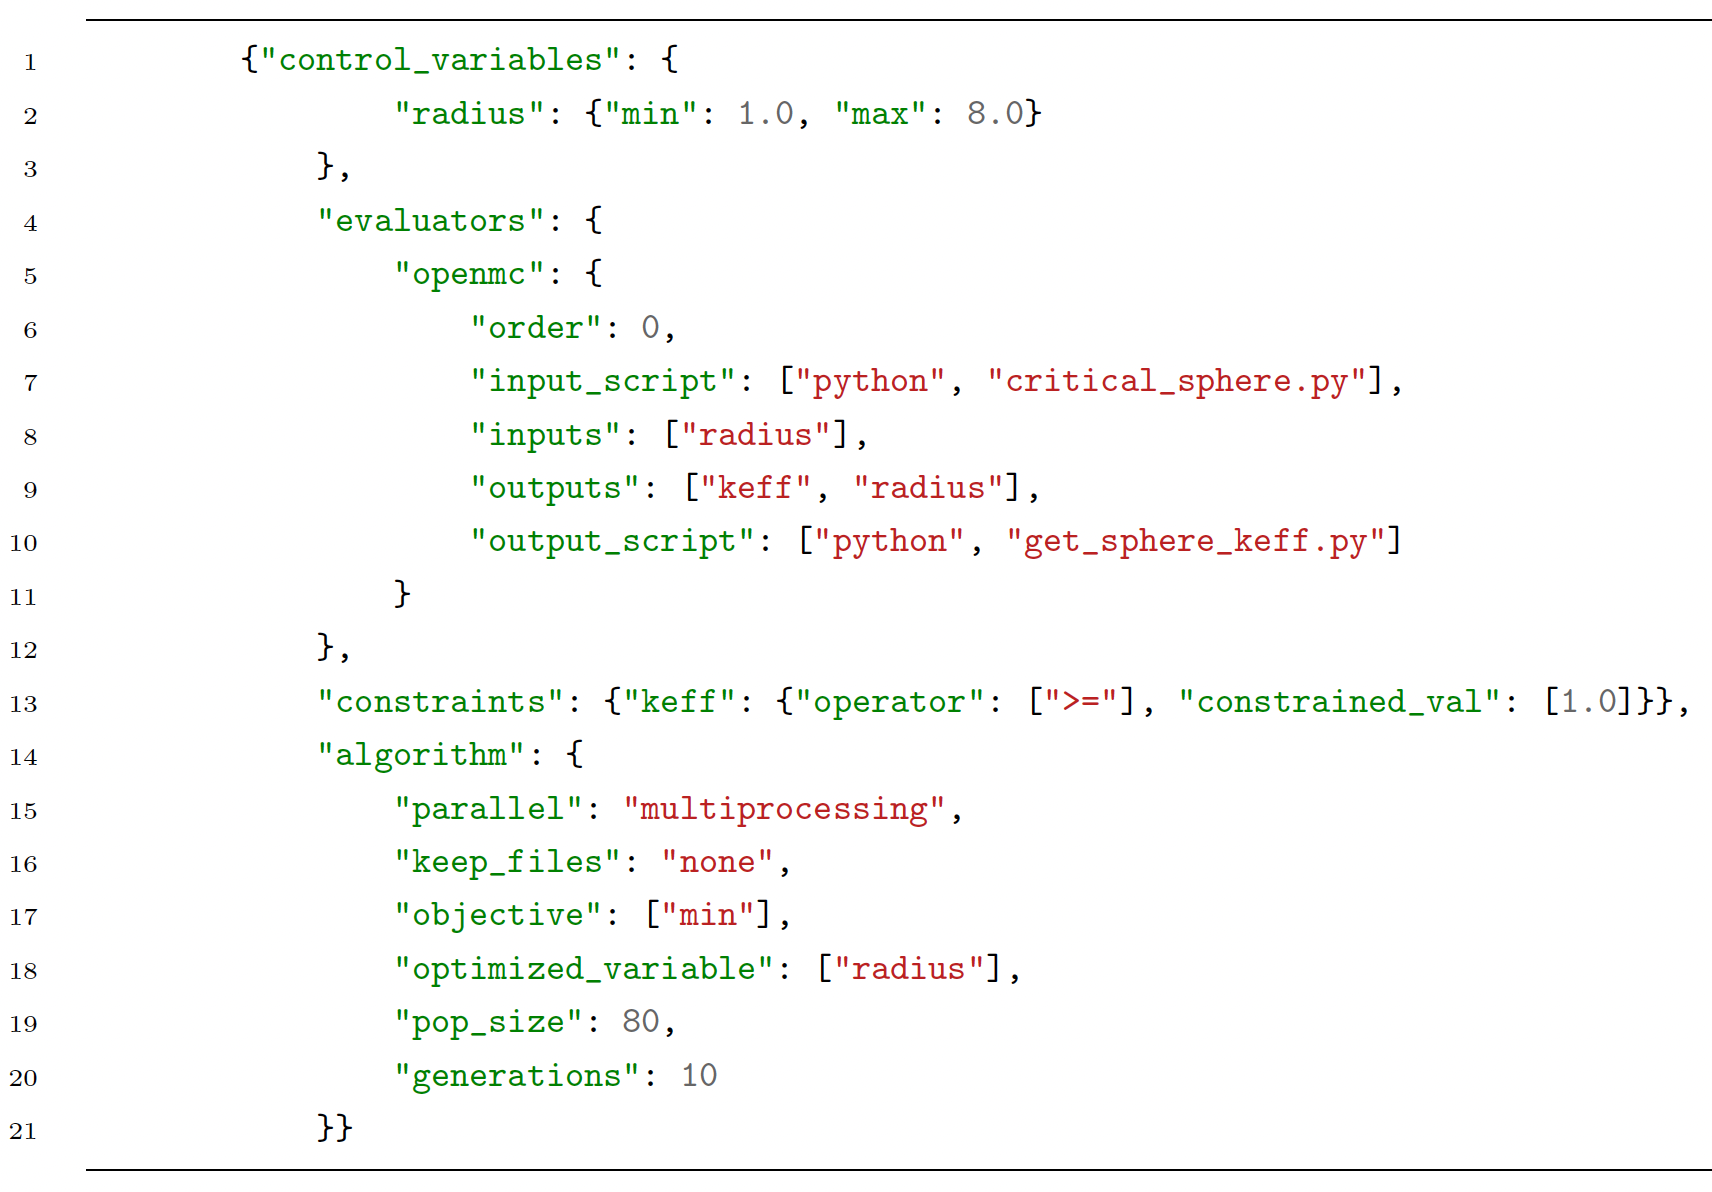
\includegraphics[width=0.49\linewidth]{figures/rollo-verify-file.png} 
        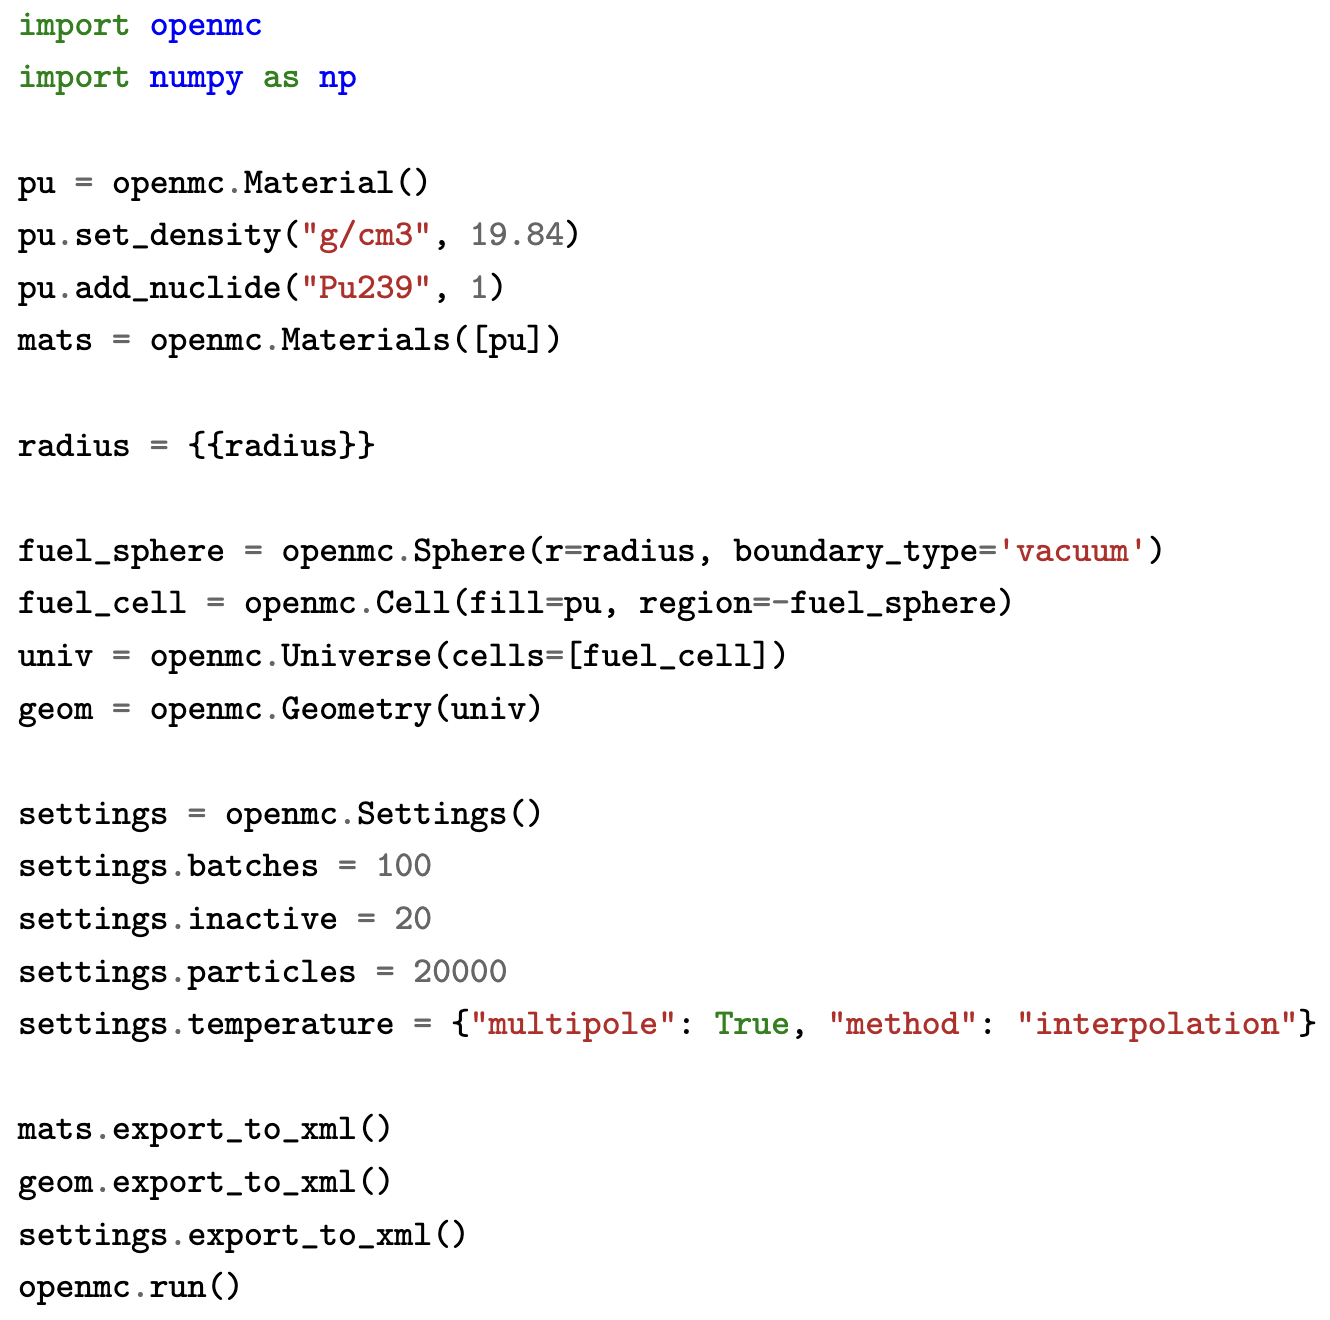
\includegraphics[width=0.49\linewidth]{figures/rollo-verify-file2.png}
        \caption{ROLLO $^{239}Pu$ Critical Bare Sphere Input File.}
    \end{figure}
\end{frame}

\begin{frame}
    \frametitle{AHTR Plank Geometry}
    A sine distribution governs TRISO packing fraction distribution: 
    \begin{align}
        \rho_{TRISO}(\vec{x}) &= \left(\textbf{a}\cdot sin(\textbf{b}\cdot x + \textbf{c}) + 2\right) \cdot NF \nonumber
    \end{align}
    \begin{figure}
        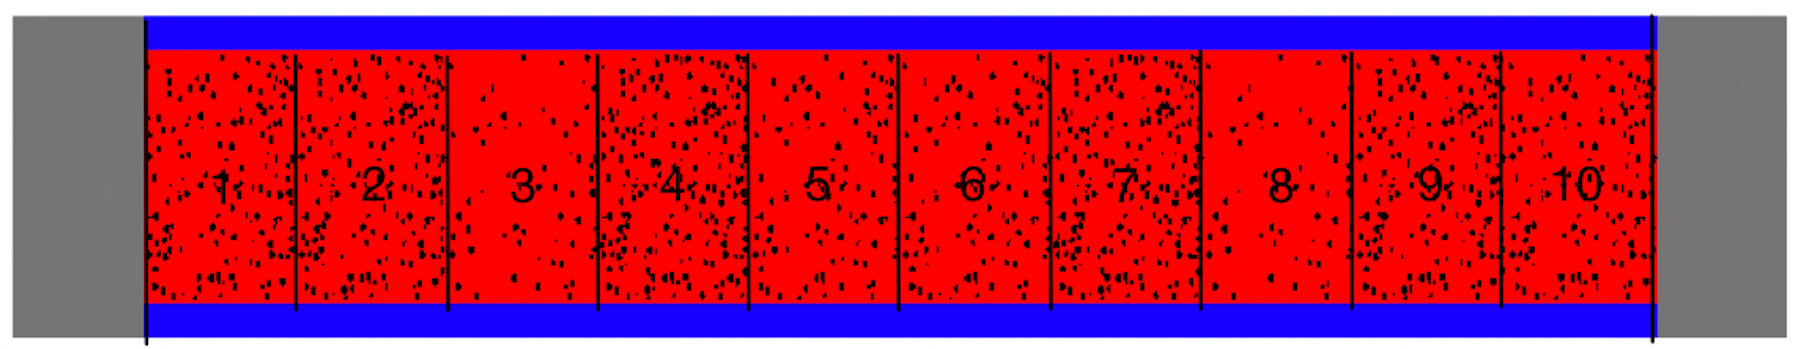
\includegraphics[width=0.9\linewidth]{../docs/figures/straightened_plank.png} 
        \caption{Straightened AHTR Plank with 10 fuel cells with random TRISO packing.}
    \end{figure}
    $r_{top}$ and $r_{bot}$ control coolant channel shape: 
    \begin{figure}
        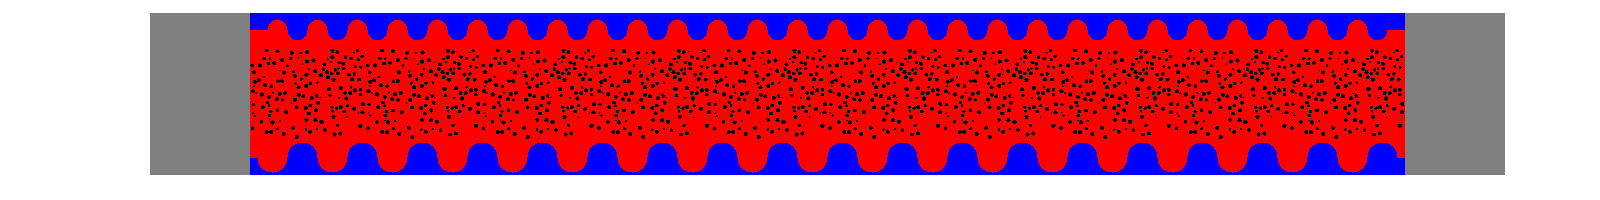
\includegraphics[width=\linewidth]{../docs/figures/coolant-channel-shape.png} 
        \caption{AHTR Plank with coolant channel shape variation, $r_{top}$ = 0.2cm and 
        $r_{bot}$ = 0.3cm.}
    \end{figure}
\end{frame}

\begin{frame}
    \frametitle{Simulation a-3b hypervolume}
    \begin{table}
        \caption{Simulation a-3b hypervolume values at each generation.}
        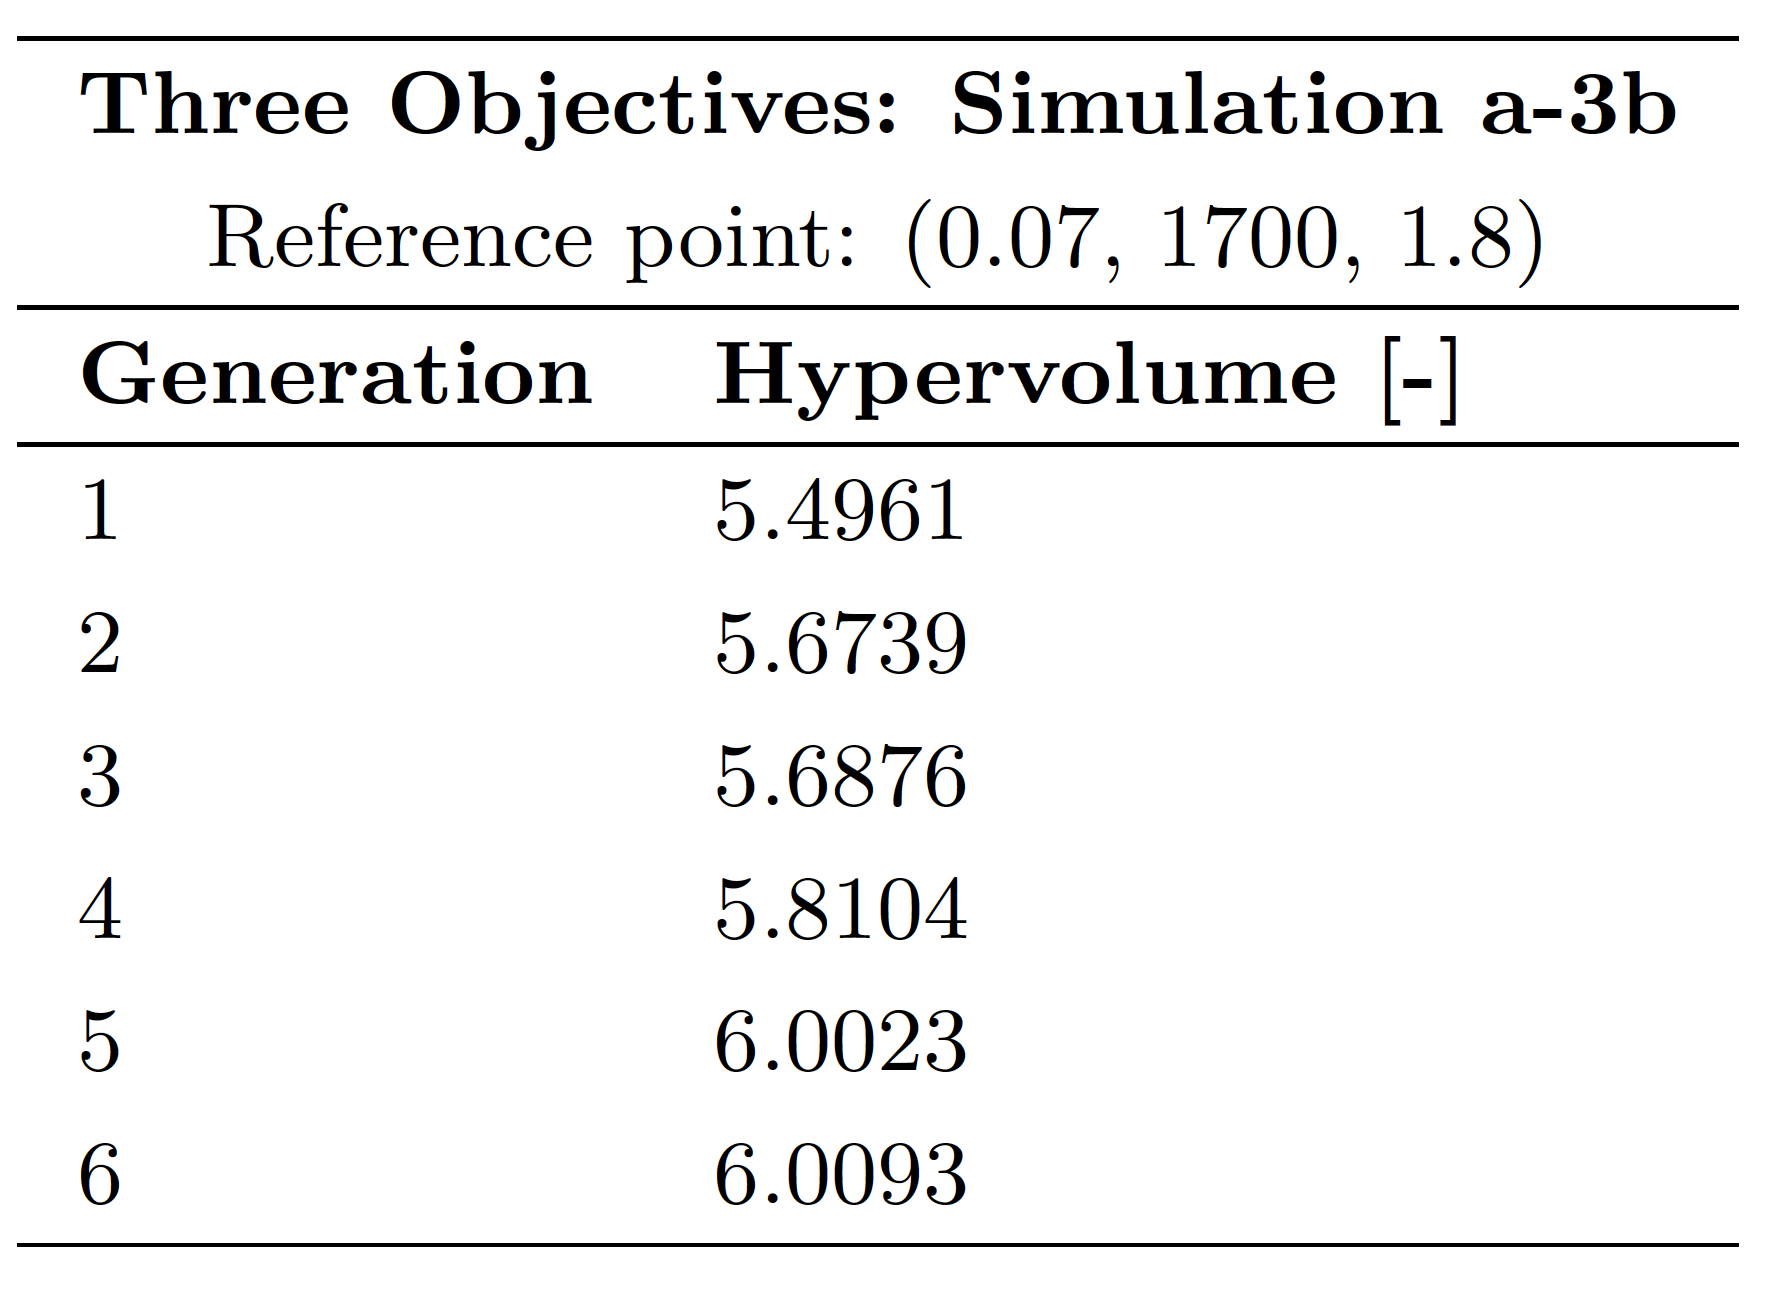
\includegraphics[width=0.4\linewidth]{figures/a-3b-hypervolume.png} 
    \end{table}

    For each optimization simulation, I must balance convergence and computational cost.

    The hypervolume is calculated by finding the volume between the reference point and 
    the objective values of the Pareto front's reactor models (bigger hypervolume = 
    more converged solution).

    I determine if convergence criteria is met by evaluating if the difference between 
    generations' hypervolume values are getting smaller.
\end{frame}